\begin{infocard}{Polígonos}

    Un \textbf{polígono} es una figura plana de muchos ángulos y con $n$ lados rectos

    \tcblower

    Un \textbf{polígono regular} es un polígono cuyos lados miden lo mismo.

    \begin{center}
        \newdimen\R
        \R=0.8cm
        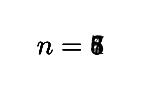
\begin{tikzpicture}
            \draw (0:\R) \foreach \x  in {120,240} {
                    -- (\x:\R)
                } -- cycle (90:\R) node[above] {$n=3$} ;
            \draw[xshift=2.5\R] (0:\R) \foreach \x in {90,180,...,359} {
                    -- (\x:\R)
                } -- cycle (90:\R) node[above] {$n=4$} ;
            \draw[xshift=5.0\R] (0:\R) \foreach \x in {72,144,...,359} {
                    -- (\x:\R)
                } -- cycle (90:\R) node[above] {$n=5$} ;
            \begin{scope}[yshift=-3\R]
                \draw (0:\R) \foreach \x in {60,120,...,359} {
                        -- (\x:\R)
                    }-- cycle (90:\R) node[above] {$n=6$} ;

                % 360/7 = 51.4286 For PGF v < 1.18 we have to round to the nearest
                % integer. Newer version support fractional angle values.
                % For a more accurate result use the sequence
                % {51, 103, 154, 206, 257, 309}
                %
                \draw[xshift=2.5\R] (0:\R) \foreach \x in {51.4286,102.8571,...,359} {
                        -- (\x:\R)
                    }-- cycle (90:\R) node[above] {$n=7$} ;
                \draw[xshift=5.0\R] (0:\R) \foreach \x in {45,90,...,359} {
                        -- (\x:\R)
                    } -- cycle (90:\R) node[above] {$n=8$} ;
            \end{scope}
        \end{tikzpicture}
    \end{center}

    %     \DrawLine

    %     \begin{center}\textbf{}\end{center}




\end{infocard}